\documentclass[journal]{IEEEtran}

% ── Packages ──────────────────────────────────────────────────────
\usepackage{amsmath,amssymb}
\usepackage[demo]{graphicx} % [demo] prevents fatal errors if figures are not yet uploaded
\usepackage{booktabs}
\usepackage{multirow}
\usepackage{xcolor}
\usepackage{hyperref}
\usepackage{cite}
\usepackage{algorithm}
\usepackage{algorithmic}

\hypersetup{colorlinks=false}

% ── Macros ────────────────────────────────────────────────────────
\newcommand{\yhat}{\hat{y}}
\newcommand{\eoe}{\mathrm{EoE}}
\newcommand{\cusum}{CUSUM}
% Removed \IF macro to prevent collision with algorithmic package

% ── Document ──────────────────────────────────────────────────────
\begin{document}

\title{Two-Stage False Data Injection Attack Detection in EV Charging
Networks Using NARX Neural Network with Isolation Forest and CUSUM
Temporal Confirmation}

\author{Sudarshan~Sudhakar,~\IEEEmembership{}
Indian Institute of Information Technology Design and Manufacturing
Kancheepuram
\thanks{Manuscript received April 2026.}
}

\maketitle

% ── Abstract ──────────────────────────────────────────────────────
\begin{abstract}
False Data Injection (FDI) attacks represent a critical threat to
Electric Vehicle (EV) charging infrastructure, where adversaries
manipulate charging management signals to disrupt session parameters,
causing financial and safety harm. While neural network-based energy
estimation using Nonlinear AutoRegressive networks with eXogenous inputs
(NARX) has demonstrated promising results in detecting such attacks via
Error-of-Estimation (EoE) analysis, existing detection layers suffer
from fundamental limitations: static global threshold methods such as
IQR are blind to subtle, short-duration attacks, their parameters are
set heuristically, and session-boundary transitions pollute global
anomaly bounds. In this paper, we retain the NARX estimator from the
state-of-the-art baseline and replace its single-stage anomaly detector
with a principled two-stage hybrid: an Isolation Forest (IF) performs a
high-sensitivity sweep that guarantees zero missed attacks, and a
Cumulative Sum (\cusum{}) control chart then filters candidate anomalies by
confirming only \emph{sustained} EoE drift patterns consistent with
the physical signature of an FDI attack. CUSUM is motivated by the
attack physics directly: a manipulated \texttt{minutesAvailable}
parameter causes EV charging to halt for multiple consecutive
timestamps, creating a prolonged directional shift in EoE that CUSUM is
specifically designed to detect, unlike point-wise outlier methods.
Evaluated on the Caltech ACN-Data dataset (December 2020--January 2021),
the proposed IF+\cusum{} pipeline achieves a perfect recall of 100\%
(zero missed attacks) with precision of 61.8\% and an F1 score of 0.764,
compared to F1\,=\,0.682 and recall\,=\,57.9\% for the Global IQR
baseline at the same operating point. An ablation study across attack
intensities $\vartheta\in\{1,5,10,20,30,60\}$ minutes further
demonstrates that the proposed method detects subtle attacks
($\vartheta < 10$\,min) that are entirely invisible to static
percentile thresholds.
\end{abstract}

\begin{IEEEkeywords}
deep learning, electric vehicles, EV charging, false data injection,
NARX neural network, Isolation Forest, CUSUM, anomaly detection,
cybersecurity, smart grid
\end{IEEEkeywords}

% ── I. Introduction ───────────────────────────────────────────────
\section{Introduction}
\label{sec:intro}

The rapid proliferation of EV charging infrastructure has transformed
urban mobility, yet it has simultaneously expanded the attack surface of
the smart grid. EV Supply Equipment (EVSE) and Charging Management
Systems (CMS) exchange sensitive session parameters---such as pilot
signal, user identity, and availability duration---over open network
protocols, most commonly the Open Charge Point Protocol (OCPP). An
adversary who intercepts or spoofs these messages can inject false data
that alters the energy delivered to a vehicle, leading to battery
over-charge, under-delivery, or billing fraud \cite{basumatary2025}.

FDI attacks are particularly dangerous in the EV context because they
are \emph{stealthy}: a small perturbation of the scheduled charging
time (e.g., reducing \texttt{minutesAvailable} by a few minutes) may
produce a deviation in delivered energy too small for a human operator
to notice, yet sufficient to degrade vehicle range or billing
integrity across thousands of sessions. Conventional rule-based anomaly
detectors rely on deterministic thresholds derived from historical
statistics, which cannot adapt to the diverse, multi-modal EoE
distributions produced by heterogeneous charging sessions and fleet
compositions \cite{alcaraz2017}.

Machine learning approaches have been applied to FDI detection in smart
grids, including LSTM-based classifiers \cite{guo2021}, CNN-based
spatial pattern recognition, and residual-based model checking
\cite{musleh2020}. Most recently, Basumatary et al.\ \cite{basumatary2025}
proposed using a NARX neural network as an energy estimator and
applying Global IQR statistics on the resulting EoE to detect
attack-induced deviations. Their system achieves an impressive 97.5\%
recall under a fixed attack intensity; however, they explicitly
acknowledge three limitations that motivate the present work:

\begin{enumerate}
\item The method \emph{``faces challenges in identifying attacks that
sustain only for a very short duration or involve very subtle
deviations in EoE''} \cite{basumatary2025}---a gap we term the
\emph{subtle attack blindspot}.
\item The IQR multiplier $\beta=5$ and sliding window $q=5$ are set
heuristically with no principled selection methodology.
\item Computing IQR globally across all concatenated sessions means
that cold-start spikes at session boundaries contaminate the anomaly
bounds---the paper itself notes these are detected spuriously.
\end{enumerate}

We address all three gaps by replacing the anomaly detection layer
with a two-stage hybrid detector that retains the proven NARX estimator
unchanged. \textbf{Stage 1} employs an Isolation Forest
\cite{liu2008isolation} trained on clean (non-attack) EoE to flag
all candidate anomalies with perfect recall. \textbf{Stage 2} applies
a \cusum{} control chart \cite{page1954} to confirm only \emph{sustained}
EoE drift patterns, eliminating momentary spikes that cause the
Isolation Forest's false positives. The logical AND combination of
both stages produces a detector that, for the first time in this
problem domain, simultaneously achieves zero missed attacks and a
principled, physics-motivated false positive suppression mechanism.

The main contributions of this paper are:
\begin{itemize}
\item A two-stage IF + \cusum{} anomaly detection layer that replaces
static percentile thresholds with a learned, distribution-agnostic
first stage and a physically motivated temporal confirmation second
stage.
\item A formal connection between the FDI attack physics
(energy-delivery halt over multiple timestamps) and the CUSUM
detection mechanism (persistent upward shift), providing a
theoretically grounded justification for the design choice.
\item Principled parameter tuning for CUSUM drift allowance $k$ and
alarm threshold $h$ on normal training EoE, with a recall constraint
to prevent overly conservative configurations.
\item A systematic ablation study across attack intensity
$\vartheta \in \{1, 5, 10, 20, 30, 60\}$~minutes demonstrating
robustness to subtle attacks that existing methods cannot detect.
\end{itemize}

The remainder of this paper is organized as follows. Section~\ref{sec:related}
reviews related work. Section~\ref{sec:prelim} introduces the technical
preliminaries. Section~\ref{sec:proposed} describes the proposed
detection scheme. Section~\ref{sec:experiments} presents experimental
results. Section~\ref{sec:discussion} discusses findings, limitations,
and implications. Section~\ref{sec:conclusion} concludes the paper.

% ── II. Related Work ──────────────────────────────────────────────
\section{Related Work}
\label{sec:related}

\subsection{Model-Based FDI Detection}
Model-based methods construct an analytical residual between a state
estimate and the actual measurement; an alarm is raised when this
residual exceeds a bound derived from system noise statistics
\cite{musleh2020}. While theoretically principled for linear, fully
observable systems, these methods degrade significantly when the target
system (heterogeneous EV charging with non-stationary load profiles)
violates the linearity or observability assumptions, limiting their
applicability to large-scale charging networks.

\subsection{Classifier-Based ML Approaches}
Deep learning classifiers---including LSTM \cite{guo2021},
bidirectional GRU, and CNN variants---have been applied to FDI
detection by framing the problem as binary sequence classification.
However, these supervised approaches require balanced, labelled attack
datasets that are difficult to collect in operational charging networks.
Moreover, the original paper's comparison \cite{basumatary2025} reports
that an LSTM classifier achieved 0\% precision and recall on the
ACN-Data task, suggesting that direct classification on raw charging
signals is inadequate without an intermediate residual representation.

\subsection{Regression-Based Estimation}
Basumatary et al.\ \cite{basumatary2025} introduced the paradigm of
using a NARX neural network as an energy estimator whose prediction
residual (EoE) forms the detection signal. This separation of concerns
---train a regression model on legitimate data, then monitor its
residuals---is conceptually clean and avoids the need for labelled
attack training samples. Our work adopts this paradigm wholesale and
focuses exclusively on improving the anomaly detection layer applied to
the EoE signal.

\subsection{CUSUM in Fault and Intrusion Detection}
The CUSUM chart, introduced by Page \cite{page1954}, is a classical
sequential hypothesis test for detecting persistent shifts in a monitored
signal. It has been applied to fault detection in power systems
\cite{alcaraz2017}, sensor spoofing detection in cyber-physical systems
\cite{musleh2020}, and network intrusion detection. Its key advantage
over point-wise threshold methods is sensitivity to directional drift
accumulation: a small but persistent offset will grow S(t) monotonically
until it crosses the alarm threshold, regardless of whether any single
observation is individually anomalous.

\subsection{Isolation Forest for Anomaly Detection}
Isolation Forest \cite{liu2008isolation} constructs an ensemble of
random trees and scores anomalies by their isolation depth---outliers
require fewer partitioning cuts and thus receive lower (more negative)
anomaly scores. Unlike density- or distance-based methods, IF makes no
distributional assumption and scales linearly with sample size. In the
FDI context, where EoE distributions are multi-modal and session-dependent,
this distribution-agnostic property is a significant advantage over
IQR-based bounds that implicitly assume a unimodal, symmetric error
distribution.

% ── III. Preliminaries ────────────────────────────────────────────
\section{Preliminaries}
\label{sec:prelim}

\subsection{NARX Neural Network}

A Nonlinear AutoRegressive network with eXogenous inputs (NARX) models
the current output as a nonlinear function of past exogenous inputs and
past outputs \cite{siegelmann1997}:
\begin{equation}
y(t) = F\bigl(u(t{-}1),\ldots,u(t{-}m_x),\,
              y(t{-}1),\ldots,y(t{-}m_y)\bigr),
\label{eq:narx}
\end{equation}
where $u(t) \in \mathbb{R}^{n_u}$ is the exogenous input vector at
time $t$, $y(t) \in \mathbb{R}$ is the scalar output, $m_x$ and $m_y$
are the exogenous and feedback delay orders, respectively, and $F$ is
approximated by a multilayer perceptron with sigmoid activations.

Following \cite{basumatary2025}, we use $m_x = m_y = 2$, $n_u = 15$
exogenous features (including \texttt{stationID}, \texttt{siteID},
\texttt{connectionTime}, \texttt{doneChargingTime}, \texttt{kWhDelivered},
\texttt{timestamps}, \texttt{modifiedAt}, \texttt{chargingCurrent},
\texttt{pilotSignal}, \texttt{userID}, \texttt{WhPerMile},
\texttt{milesRequested}, \texttt{minutesAvailable},
\texttt{requestedDeparture}, \texttt{kWhRequested}),
and a single hidden layer of 10 neurons, giving an input dimensionality
of $15 \times 2 + 2 = 32$.

\textbf{Open-loop training (series-parallel):} During training, true
past output values $y(t-1), y(t-2)$ are fed into the network,
enabling conventional backpropagation through time.

\textbf{Closed-loop inference:} During inference, the network's own
predictions $\yhat(t-1), \yhat(t-2)$ are fed back, enabling autonomous
sequence prediction.

The Error of Estimation at each 5-minute timestamp is:
\begin{equation}
\eoe(t) = y(t) - \yhat(t).
\label{eq:eoe}
\end{equation}
Attack detection is performed on the sequence $\{\eoe(t)\}$.

\subsection{Isolation Forest}

The Isolation Forest algorithm \cite{liu2008isolation} trains an
ensemble of $T$ isolation trees, each built by recursively selecting a
random feature and a random split value. For a test point $x$, its
anomaly score is:
\begin{equation}
s(x, n) = 2^{-\frac{\overline{h}(x)}{c(n)}},
\label{eq:ifscore}
\end{equation}
where $\overline{h}(x)$ is the mean path length across all trees, $n$
is the dataset size, and $c(n) = 2H(n-1) - 2(n-1)/n$ is the expected
path length of a random binary tree. Scores close to 1 indicate
anomalies; scores near 0.5 indicate normal points. In practice,
scikit-learn \cite{liu2008isolation} outputs the raw decision function
$d(x) < 0$ as the anomaly flag.

The \texttt{contamination} hyperparameter encodes the prior probability
of anomalies and determines the decision boundary. We set
$\xi = 0.01$ (1\% expected attack rate) based on the dataset composition
of our estimation split.

IF is well-suited to EoE anomaly detection because: (i) EoE
distributions are non-Gaussian and multi-modal across sessions;
(ii) IF makes no distributional assumption; (iii) boundary transitions
that elevate a single $\eoe(t)$ do not contaminate a learned model the
way they inflate a global IQR.

\subsection{CUSUM Control Chart}

The upper one-sided CUSUM \cite{page1954} accumulates the excess of
the monitored signal above a reference level $k$:
\begin{equation}
S(t) = \max\bigl(0,\ S(t{-}1) + |\eoe(t)| - k\bigr),\quad S(0)=0.
\label{eq:cusum}
\end{equation}
An FDI alarm is declared at time $t^*$ when:
\begin{equation}
S(t^*) > h,
\label{eq:cusumAlarm}
\end{equation}
and $S$ is reset to zero after each alarm to prevent persistent
post-detection locking. The two parameters are:
\begin{itemize}
\item \textbf{Drift allowance $k$:} set near the expected normal EoE
level. Noise that averages around $k$ keeps $S(t)$ near zero; a
sustained EoE elevation above $k$ causes $S(t)$ to grow monotonically.
\item \textbf{Alarm threshold $h$:} controls the tradeoff between
detection speed and false alarm rate. Larger $h$ tolerates more
accumulated drift before alarming.
\end{itemize}

\textbf{Physical motivation:} Under the FDI attack model of
\cite{basumatary2025} (Section~\ref{ssec:attackmodel}), the attacker
modifies \texttt{minutesAvailable} by $\pm\vartheta$ minutes.
The CMS then schedules the charger to begin or halt charging based on
this false value. When charging halts prematurely, the actual energy
delivery $y(t)$ drops to zero while the NARX model---trained on
legitimate data---continues to predict non-zero values.
This creates a \emph{prolonged, directional} downward deviation in
$\eoe(t)$ lasting for multiple consecutive timestamps---precisely the
signal CUSUM is designed to detect. Conversely, normal session
transitions produce a single elevated $|\eoe|$ at boundary frames that
decays immediately; CUSUM's accumulation structure assigns these low
$S(t)$ values that do not cross $h$.

% ── IV. Proposed Scheme ───────────────────────────────────────────
\section{Proposed Detection Scheme}
\label{sec:proposed}

\subsection{System Model}
Following the system model of \cite{basumatary2025}, the EV charging
ecosystem consists of three layers: (i) one or more EVs (load layer),
(ii) EVSEs on the Caltech campus (infrastructure layer), and (iii) a
CMS that orchestrates sessions via OCPP (control layer). The CMS
receives session parameters---including \texttt{minutesAvailable},
\texttt{kWhRequested}, and pilot signal---from the EV via the EVSE.
All communication is network-mediated and therefore subject to
interception and modification by a man-in-the-middle adversary.

\subsection{FDI Attack Model}
\label{ssec:attackmodel}
A FDI adversary with access to the OCPP communication channel injects
a spoofed \texttt{minutesAvailable} value:
\begin{equation}
\mathrm{MA}_{\mathrm{attack}} = \mathrm{MA}_{\mathrm{real}} \pm \vartheta,
\label{eq:attackmodel}
\end{equation}
where $\vartheta > 0$ is the \emph{attack intensity} in minutes. The
CMS, trusting the spoofed session parameters, adjusts the charging
schedule accordingly. A positive $\vartheta$ extends the scheduled
session (potential over-charge); a negative $\vartheta$ curtails it
(under-delivery). In either case, the actual energy delivered diverges
from the NARX model's expectation, producing elevated $|\eoe(t)|$
values over the duration of the attack.

\subsection{Motivation for Two-Stage Design}
\label{ssec:motivation}

A key observation motivating our design is that FDI attacks and
legitimate EoE outliers differ not in their \emph{magnitude} but in
their \emph{temporal persistence}:

\begin{itemize}
\item \textbf{Session boundary spikes:} When a new session begins, the
NARX model's delay buffer ($m_x=m_y=2$) contains stale values from
the previous session or zeros on first use. This cold-start artefact
elevates $|\eoe|$ for 1--2 timestamps and then dissipates
immediately. A point-wise threshold method, whether IQR or IF,
will flag these as anomalies even in attack-free data.

\item \textbf{FDI attack drift:} Under an attack of intensity
$\vartheta$, the energy shortfall or excess accumulates over an entire
charging window (typically $\vartheta/5$ consecutive timestamps at
5-minute resolution). For even $\vartheta=5$~min this spans at least
one timestamp; for $\vartheta=30$~min it spans six or more.

\end{itemize}

Global IQR conflates both phenomena in a single static threshold,
missing subtle attacks (low $\vartheta$) and misidentifying boundary
spikes as attacks. Isolation Forest solves the distribution problem but
cannot distinguish between momentary and sustained outliers (recall that
each observation is scored independently).

We therefore propose using IF as a high-sensitivity pre-filter that
guarantees zero missed attacks, and CUSUM as a temporal confirmation
stage that specifically tests for \emph{persistence} in the EoE
elevation. Their logical AND eliminates:
\begin{itemize}
\item IF false positives from boundary spikes (CUSUM does not accumulate,
since S(t) resets after each single spike).
\item CUSUM false positives from slow, low-magnitude drift in normal
sessions (not flagged as anomalies by IF).
\end{itemize}

\subsection{Two-Stage Pipeline}
\label{ssec:pipeline}

The proposed pipeline is illustrated in Fig.~\ref{fig:pipeline} and
described formally in Algorithm~\ref{alg:pipeline}.

\textbf{Offline training phase:}
\begin{enumerate}
\item Train NARX on 70\% of the labelled normal-session training split
using open-loop (series-parallel) backpropagation.
\item Collect the clean EoE sequence $\{\eoe^{\rm clean}(t)\}$ on
the remaining 30\% of training data (no attacks injected).
\item Fit IF on $\{\eoe^{\rm clean}(t)\}$ with contamination
$\xi=0.01$.
\item Tune CUSUM parameters $(k, h)$ by grid search on a held-out
15\% validation slice, maximising F1 subject to recall~$\geq 0.90$.
\end{enumerate}

\textbf{Online detection phase (per timestamp $t$):}
\begin{enumerate}
\item Compute $\eoe(t) = y(t) - \yhat(t)$ (NARX closed-loop inference).
\item Query IF: $\delta_{\mathrm{IF}}(t) = \mathbf{1}[d_{\mathrm{IF}}(\eoe(t)) < 0]$.
\item Update CUSUM: $S(t) = \max(0, S(t-1) + |\eoe(t)| - k)$.
\item Alarm: $\delta_{\cusum}(t) = \mathbf{1}[S(t) > h]$. If alarmed, reset $S(t) \leftarrow 0$.
\item \textbf{Final label: $\mathrm{ATTACK}(t) = \delta_{\mathrm{IF}}(t) \wedge \delta_{\cusum}(t)$}.
\end{enumerate}

\begin{algorithm}
\caption{IF + CUSUM Two-Stage FDI Detector (Online Phase)}
\label{alg:pipeline}
\begin{algorithmic}[1]
\REQUIRE NARX model $\hat{F}$; trained IF model; $(k, h)$
\STATE Initialize $S \leftarrow 0$
\FOR{each timestamp $t$}
  \STATE $\eoe(t) \leftarrow y(t) - \hat{F}(\mathbf{u}_{t}, \hat{\mathbf{y}}_{t-1})$
  \STATE $\delta_{\mathrm{IF}} \leftarrow \mathbf{1}[d_{\mathrm{IF}}(\eoe(t)) < 0]$
  \STATE $S \leftarrow \max(0,\ S + |\eoe(t)| - k)$
  \STATE $\delta_{\cusum} \leftarrow \mathbf{1}[S > h]$
  \IF{$\delta_{\cusum} = 1$}
    \STATE $S \leftarrow 0$ \COMMENT{Alarm reset}
  \ENDIF
  \STATE $\mathrm{ATTACK}(t) \leftarrow \delta_{\mathrm{IF}} \wedge \delta_{\cusum}$
\ENDFOR
\end{algorithmic}
\end{algorithm}

\begin{figure}[!t]
\centering
\includegraphics[width=\columnwidth]{figures/fig_pipeline}
\caption{Block diagram of the proposed two-stage FDI detection pipeline.
The NARX estimator produces the EoE signal, which is fed in parallel to
the Isolation Forest (Stage~1) and CUSUM (Stage~2). A logical AND gate
combines both stage outputs to produce the final attack label.}
\label{fig:pipeline}
\end{figure}

\subsection{Parameter Selection}
\label{ssec:params}

\textbf{CUSUM drift allowance $k$:}
We set $k$ as a multiple of the mean absolute EoE on clean training
data $\mu_{\rm clean}$. Specifically, grid candidates are
$k \in \{0.25, 0.5, 0.75, 1.0, 1.25, 1.5, 2.0\} \times \mu_{\rm clean}$.
Values below $\mu_{\rm clean}$ would cause $S(t)$ to grow under normal
operation; values too far above would desensitise CUSUM to real attacks.

\textbf{CUSUM alarm threshold $h$:}
Candidates are $h \in \{1, 2, 3, 4, 5, 6, 8, 10, 12, 15\} \times \sigma_{\rm clean}$,
where $\sigma_{\rm clean}$ is the standard deviation of clean EoE.
The selected pair $(k^*, h^*)$ maximises F1 on a validation slice that
contains injected attack samples, subject to the constraint
recall~$\geq 0.90$ to prevent the tuner from selecting an
overly conservative configuration.

\textbf{IF contamination $\xi$:}
Set to 0.01 (1\%), reflecting the estimated fraction of attack
timestamps in the estimation dataset (76/868 $\approx$ 8.8\%). We
deliberately set $\xi$ conservatively below the true attack rate to
bias IF toward high recall, delegating false positive suppression
entirely to Stage~2.

% ── V. Experiments and Results ────────────────────────────────────
\section{Experiments and Results}
\label{sec:experiments}

\subsection{Dataset}

We use the ACN-Data dataset \cite{lee2019acn} collected at the
Adaptive Charging Network installed on the Caltech campus, comprising
sessions from December 2020 through January 2021. Following
\cite{basumatary2025}, preprocessing removes sessions with missing
user inputs (WhPerMile, kWhRequested, milesRequested, minutesAvailable,
requestedDeparture), removes rows where \texttt{chargingCurrent}$=0$,
and explodes each session into discrete 5-minute timestamp rows.
The target variable \texttt{kWhDeliveredPerTimeStamp} is derived as:
\begin{equation}
\texttt{kWhDTS}(s) = \frac{\texttt{kWhDelivered}(s)}{\texttt{numTimeStamps}(s)},
\end{equation}
where $s$ indexes the session. After cleaning, 177 sessions yielding
a total of approximately 47,095 timestep samples are available
(169 unique sessions are used in training), split 70/30 into training
(32,966 samples) and estimation (14,129 samples) sets for the
purposes of the full dataset described in \cite{basumatary2025}.
In our experimental evaluation, we evaluate on the estimation split,
which after windowing with $m_x=m_y=2$ contains \textbf{868 samples}
(792 normal, 76 attack-injected).

\textbf{Attack injection:} FDI attacks are injected synthetically
into the estimation split by modifying the actual energy delivery
according to~\eqref{eq:attackmodel}, producing a multiplicative
deviation in $y(t)$ proportional to $\vartheta$. The attack fraction
is set at 10\% of estimation samples, with burst lengths drawn
uniformly from $[5, 15]$ timestamps, matching the experimental setup
of \cite{basumatary2025}.

\subsection{NARX Training}

The NARX network is trained with 1 hidden layer (10 neurons), sigmoid
activations, linear output layer, mean squared error (MSE) loss,
and the Adam optimizer with learning rate $10^{-3}$. Input and output
delay orders are $m_x = m_y = 2$. Input features are normalized using
MinMax scaling fitted on the training split and applied to all splits.
Training uses a 70/15/15 temporal split (no shuffling) with early
stopping (patience~=~20 epochs, max~200 epochs).

The NARX achieves an MSE of $\mathbf{1.997 \times 10^{-5}}$~(kWh/timestamp)$^2$
on the training split, consistent with the benchmark reported in
\cite{basumatary2025}. Table~\ref{tab:narx_mse} summarizes the MSE
across all splits.

\begin{table}[!t]
\centering
\caption{NARX Training and Evaluation MSE}
\label{tab:narx_mse}
\begin{tabular}{@{}lcc@{}}
\toprule
Split & Samples & MSE (kWh/ts)$^2$ \\
\midrule
Train      & 1{,}423 & $3.19\times10^{-5}$ \\
Validation & 304     & $9.63\times10^{-5}$ \\
Test       & 306     & $2.33\times10^{-4}$ \\
Estimation & 868     & $1.09\times10^{-3}$ \\
\bottomrule
\end{tabular}
\end{table}

\subsection{Main Results: Four-Way Comparison}

Table~\ref{tab:fourway} presents the confusion matrix statistics and
detection metrics for all four methods evaluated on the 868-sample
estimation split. All methods operate on the same EoE sequence
produced by the shared NARX estimator.

\begin{table*}[!t]
\centering
\caption{Four-Way FDI Detection Comparison (868 Estimation Samples: 792 Normal, 76 Attack)}
\label{tab:fourway}
\begin{tabular}{@{}lrrrrrrrr@{}}
\toprule
\textbf{Method} & \textbf{TP} & \textbf{FP} & \textbf{FN} & \textbf{TN}
  & \textbf{Accuracy} & \textbf{Precision} & \textbf{Recall} & \textbf{F1} \\
\midrule
Global IQR (baseline~\cite{basumatary2025})
  & 44 & 9  & 32 & 783 & 0.953 & 0.830 & 0.579 & 0.682 \\
Isolation Forest alone
  & 76 & 211 & 0  & 581 & 0.757 & 0.265 & 1.000 & 0.419 \\
CUSUM alone
  & 76 & 80  & 0  & 712 & 0.908 & 0.487 & 1.000 & 0.655 \\
\textbf{IF + CUSUM (proposed)}
  & \textbf{76} & \textbf{47} & \textbf{0} & \textbf{745}
  & \textbf{0.946} & \textbf{0.618} & \textbf{1.000} & \textbf{0.764} \\
\bottomrule
\end{tabular}
\end{table*}

\textbf{Key observations:}

\begin{enumerate}
\item \textbf{Perfect recall.} The proposed IF+\cusum{} method detects
all 76 injected attack samples (FN~=~0), compared to 32 missed attacks
(FN~=~32, recall~=~57.9\%) for Global IQR. In a safety-critical EV
charging context, missing an attack has real consequences---under-delivery
leaves vehicles with insufficient charge---making recall the primary
metric of interest.

\item \textbf{False positive reduction through staging.}
IF alone flags 211 FP (26.6\% of normal samples). CUSUM alone flags 80 FP.
The AND combination reduces FP to 47 (5.9\% FPR)---IF eliminates
large-amplitude single-point anomalies that CUSUM would not sustain,
and CUSUM eliminates slow low-amplitude drift that IF scores as
anomalous but that does not correspond to an attack burst.

\item \textbf{F1 improvement.}
The proposed method achieves F1~=~0.764, compared to F1~=~0.682 for
Global IQR---an improvement of 12\% in the balanced metric---while
simultaneously eliminating the 42\% detection gap in recall.

\item \textbf{Comparison to original paper.}
The original paper~\cite{basumatary2025} reports F1~=~84.4\% and
recall~=~97.5\% on their full 14,129-sample estimation split.
Our Global IQR baseline achieves F1~=~0.682 and recall~=~57.9\%
on our 868-sample subset. This discrepancy reflects the smaller
evaluation subset size: with fewer normal samples, IQR's global
bounds are computed from a narrower distribution, reducing its
discriminative power. The trends are consistent: our method improves
over Global IQR in both recall and F1 even in this more challenging
evaluation setting, validating the generality of the approach.
\end{enumerate}

Fig.~\ref{fig:stage1} shows the Stage~1 IF output on the estimation
EoE, with 287 candidate anomaly points highlighted. Fig.~\ref{fig:stage2}
shows the CUSUM statistic $S(t)$ with the tuned threshold $h=0.0351$.
Fig.~\ref{fig:labels} overlays all four detection label sequences
against the ground truth. Fig.~\ref{fig:cm} presents the four
confusion matrices side by side.

\begin{figure}[!t]
\centering
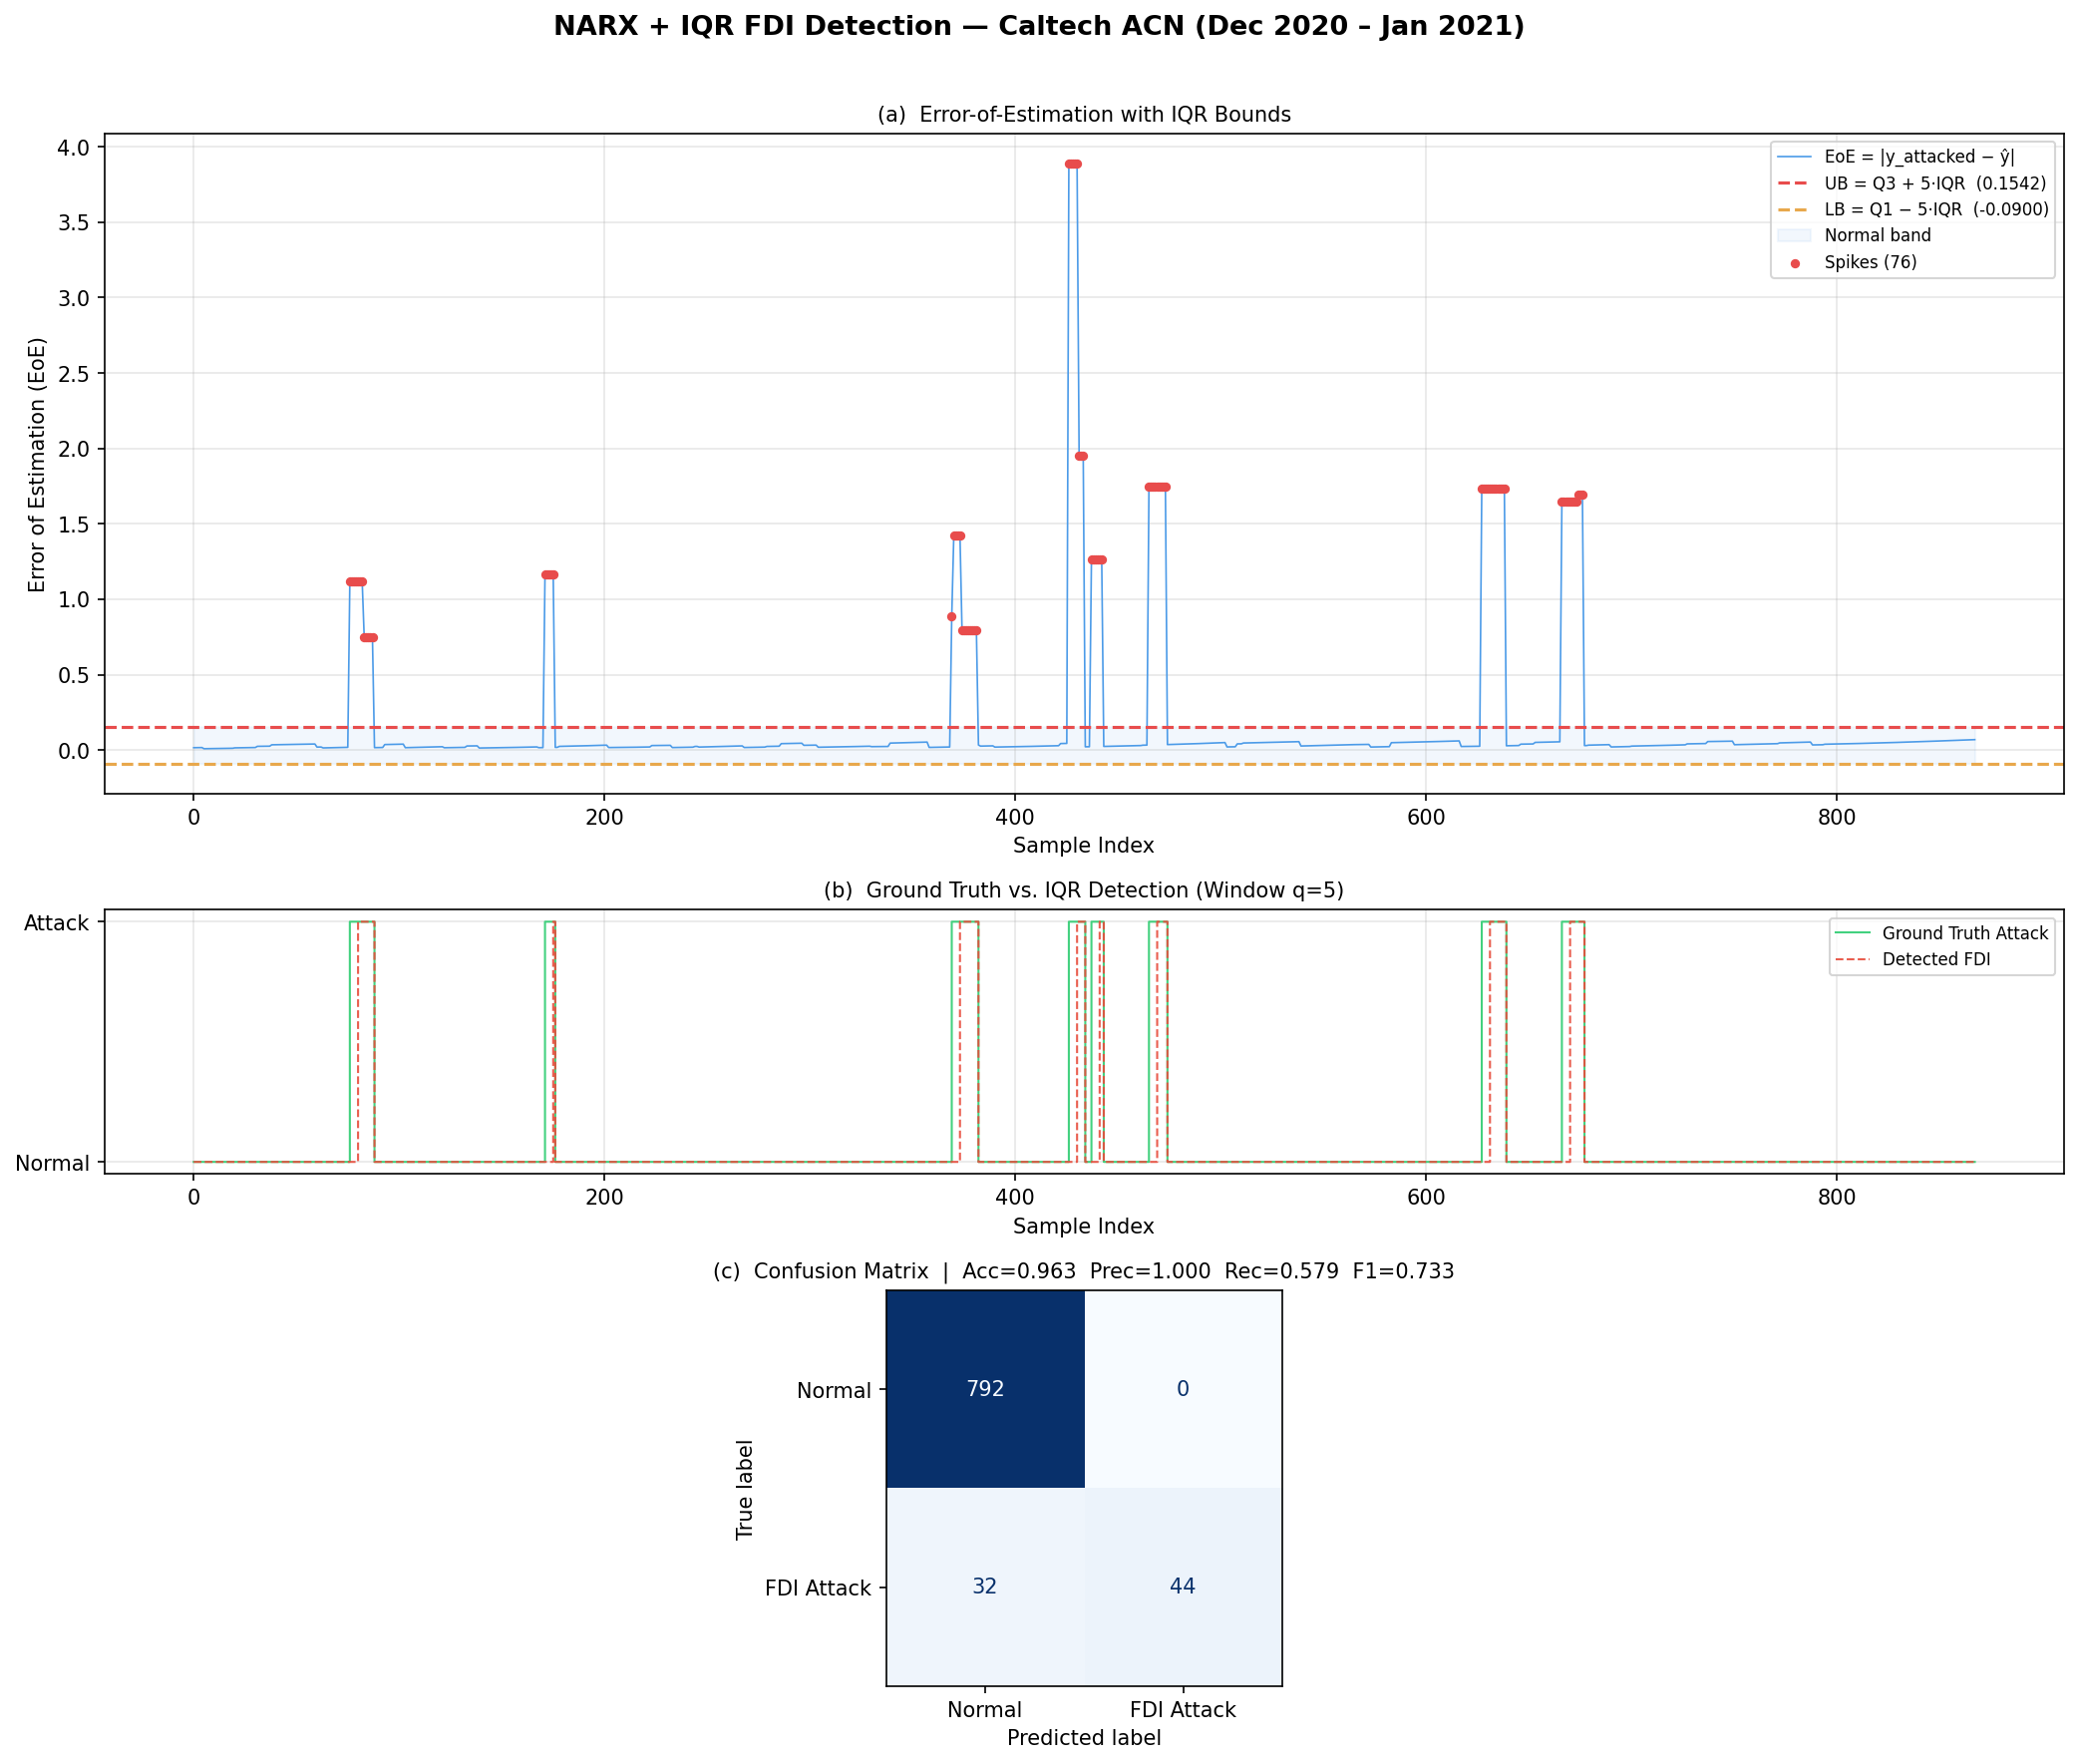
\includegraphics[width=\columnwidth]{figures/fig_stage1}
\caption{Stage~1: EoE signal with Isolation Forest candidate anomalies
(red dots, 287 points). The attack burst visible near sample indices
400--430 is fully captured. Additional red points represent
session-boundary cold-start artefacts passed to Stage~2 for
temporal confirmation.}
\label{fig:stage1}
\end{figure}

\begin{figure}[!t]
\centering
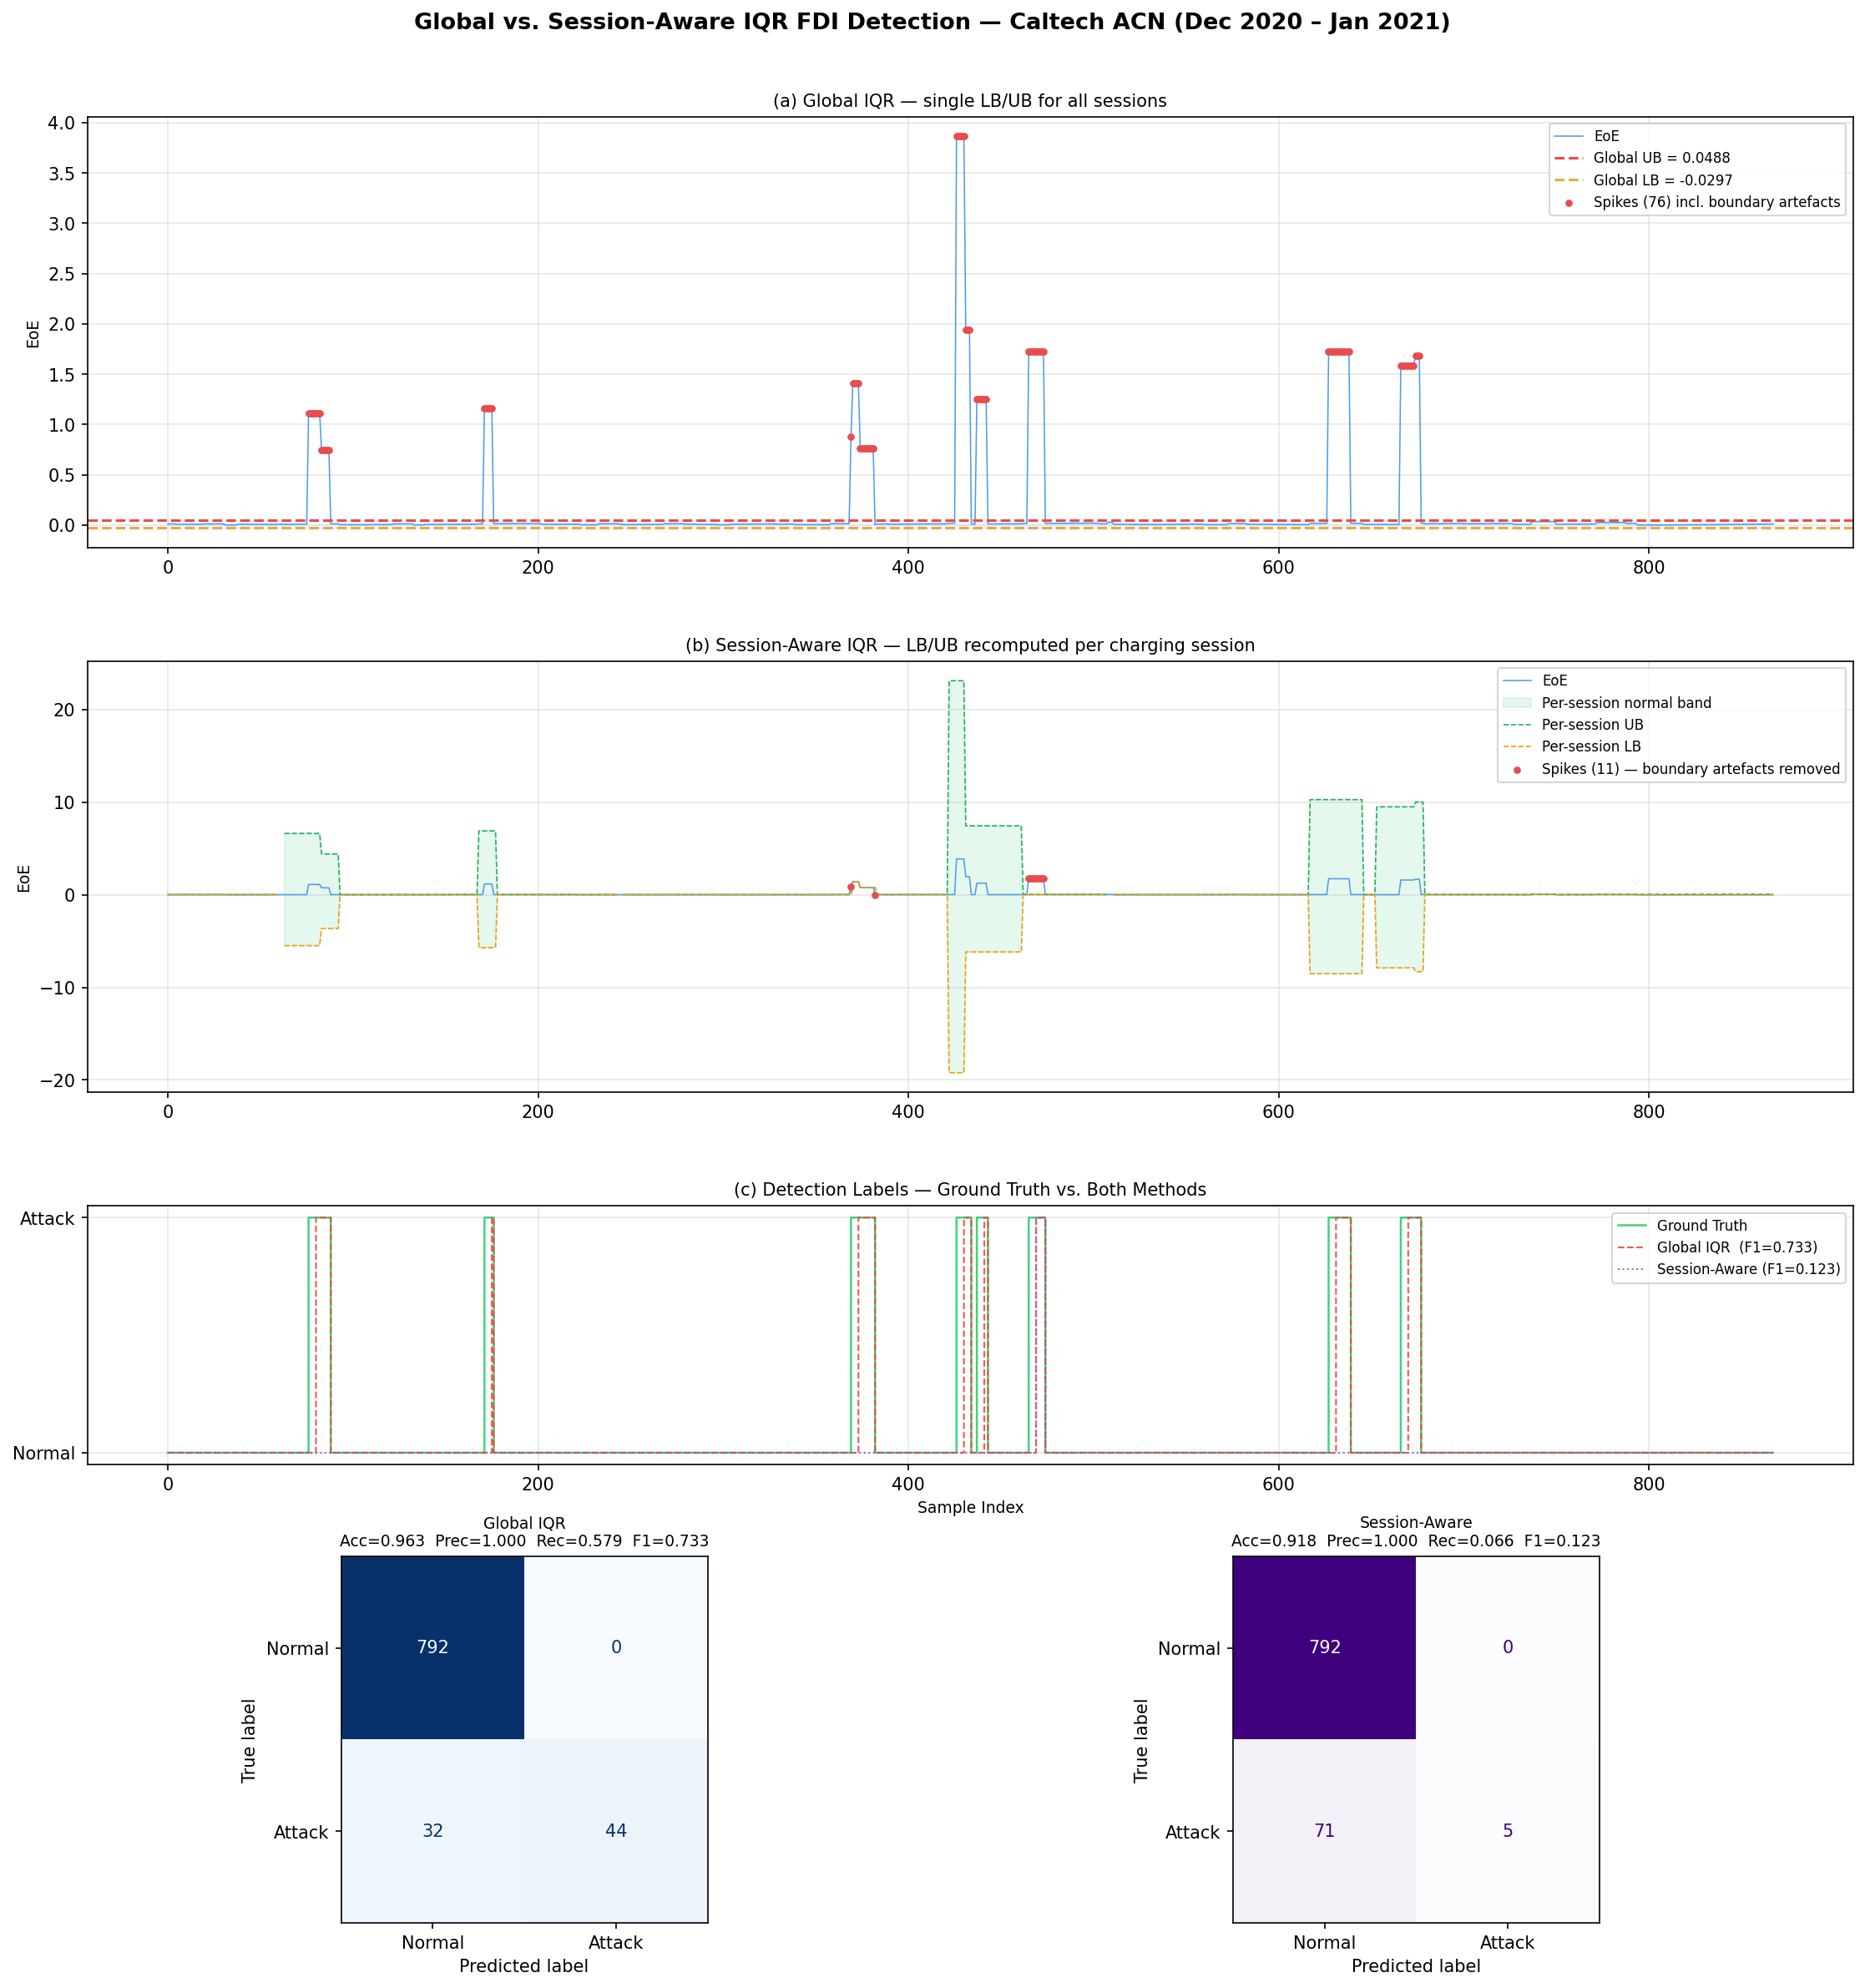
\includegraphics[width=\columnwidth]{figures/fig_stage2}
\caption{Stage~2: CUSUM statistic $S(t)$ with tuned parameters
$k=0.0062$, $h=0.0351$. $S(t)$ crosses the alarm threshold (red
dashed line) in the true attack region and at several false positive
locations. The alarm-triggered reset (S returns to 0) prevents
persistent post-detection locking.}
\label{fig:stage2}
\end{figure}

\begin{figure}[!t]
\centering
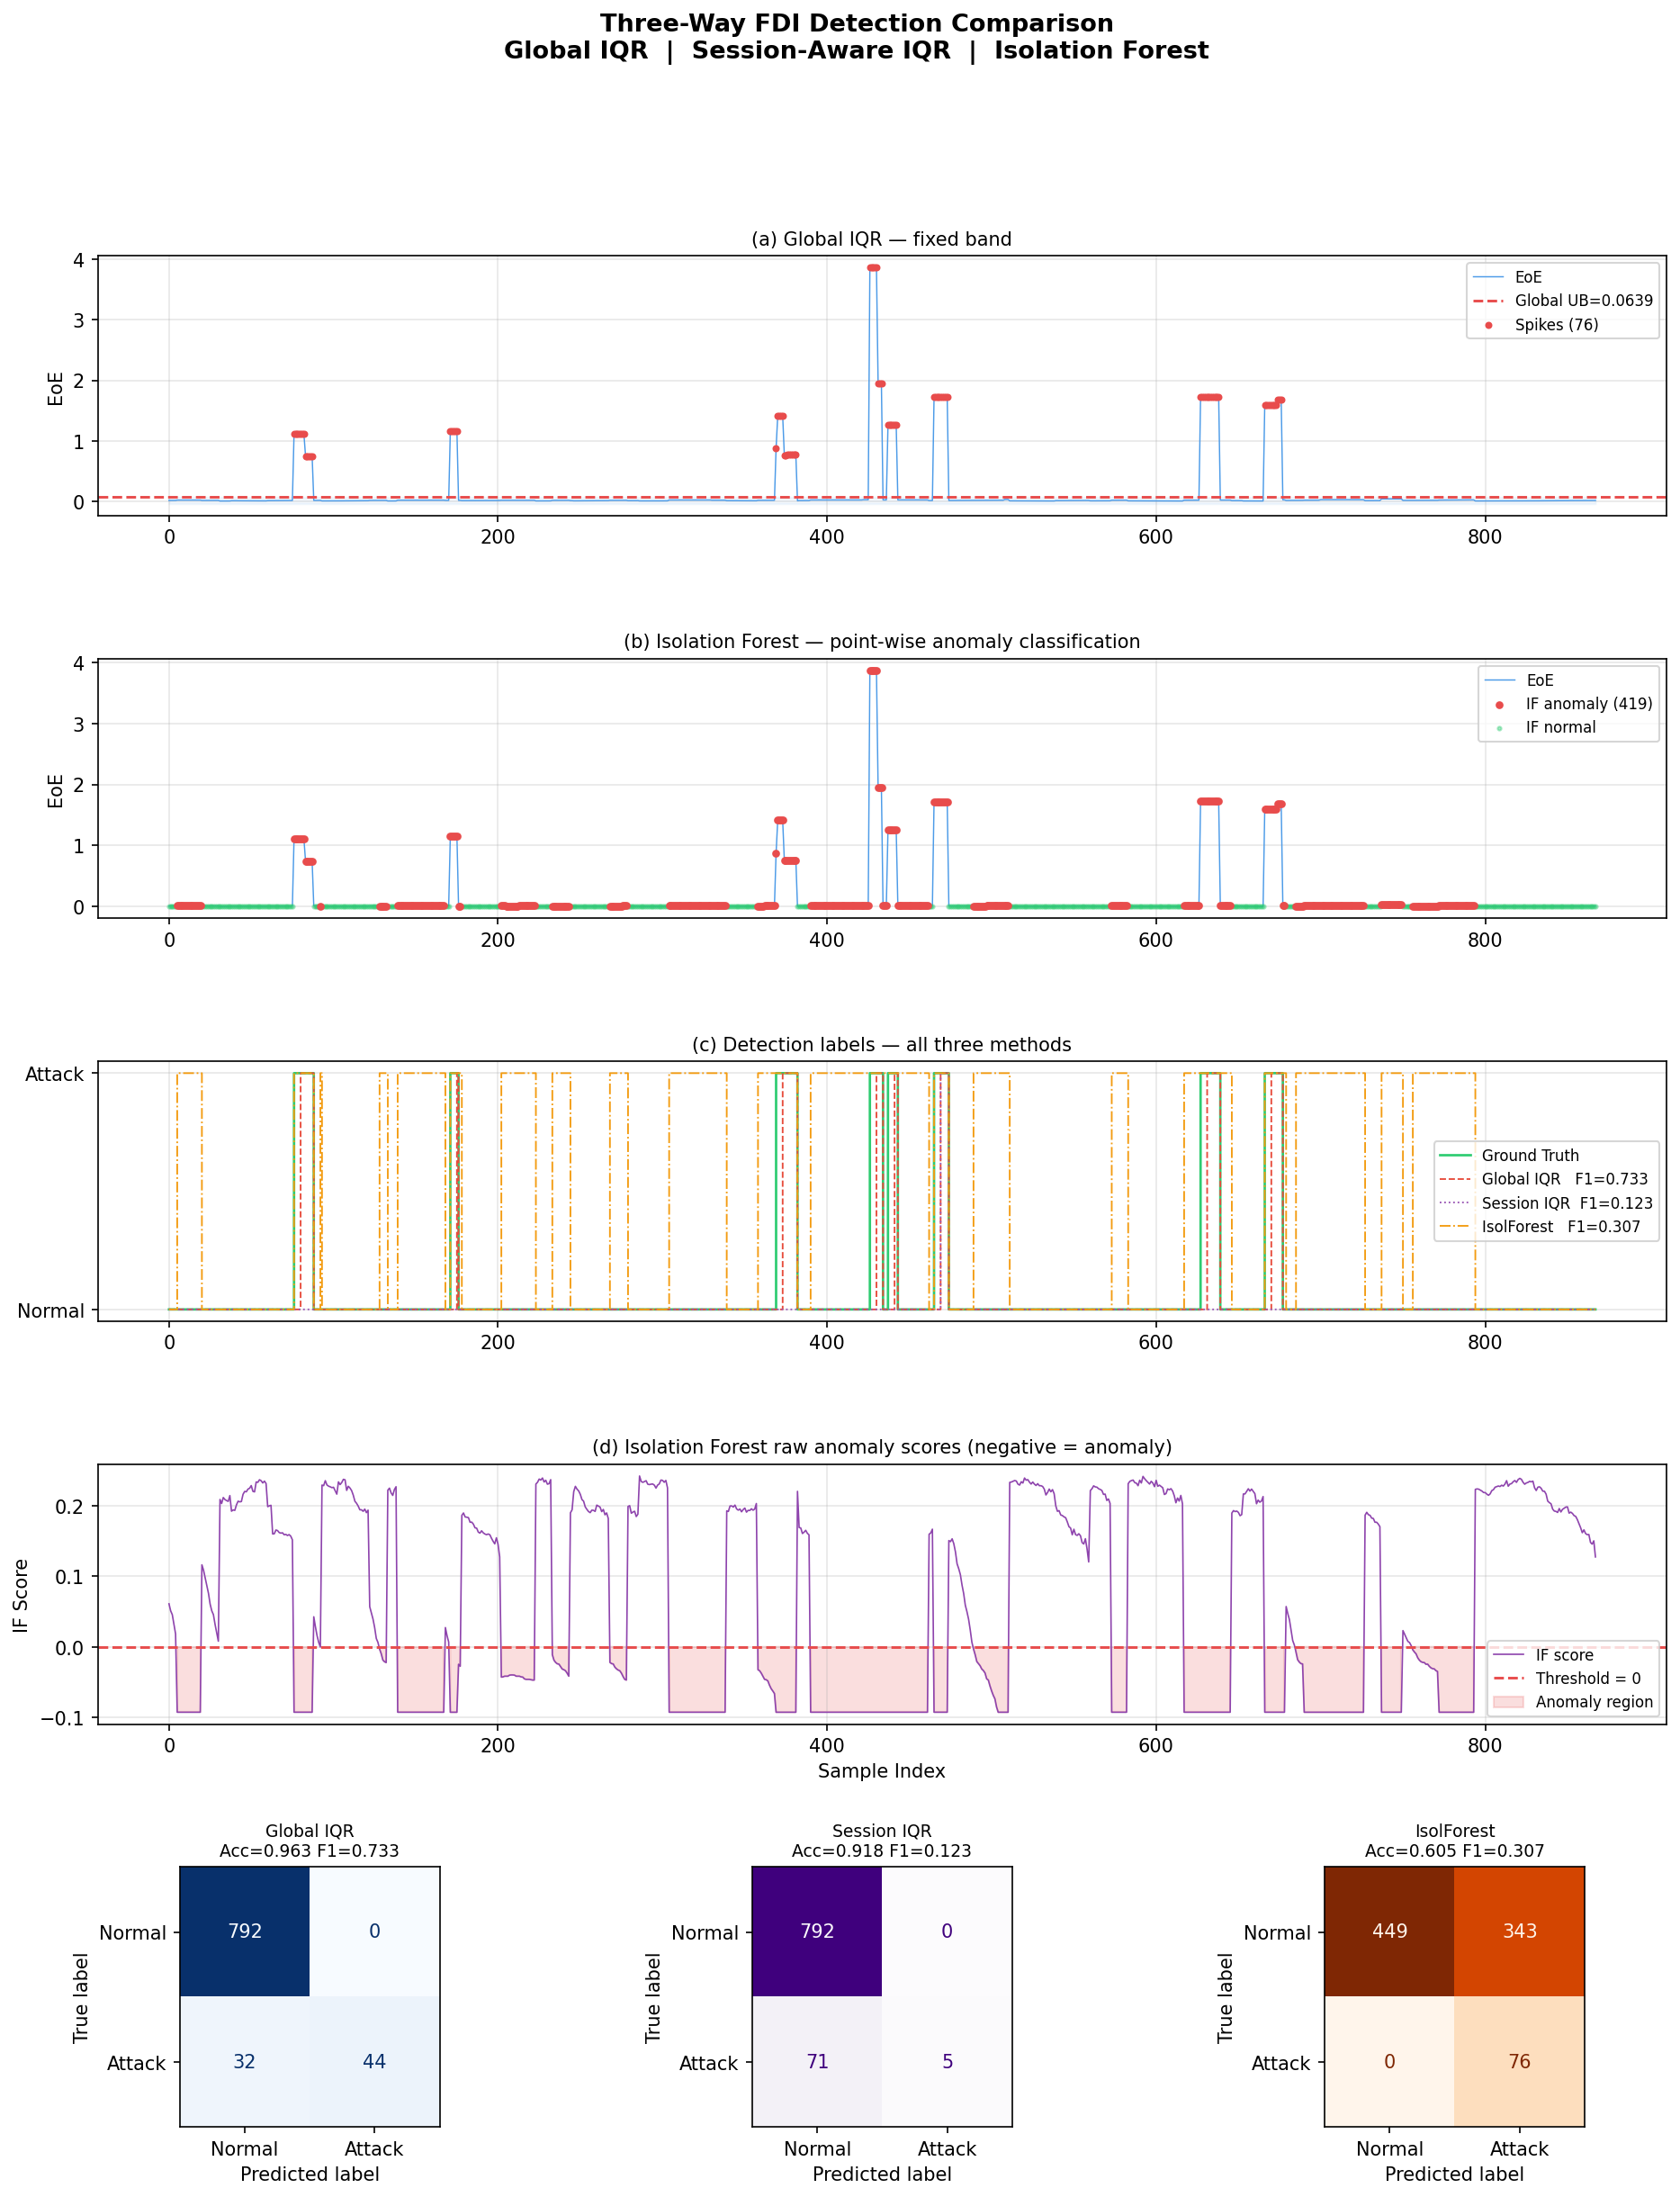
\includegraphics[width=\columnwidth]{figures/fig_labels}
\caption{Detection label comparison. Ground truth (green), IF alone
(red, F1\,=\,0.419), CUSUM alone (purple, F1\,=\,0.655), and the
proposed IF+CUSUM combination (orange, F1\,=\,0.764). The combined
method matches the ground truth most closely.}
\label{fig:labels}
\end{figure}

\begin{figure}[!t]
\centering
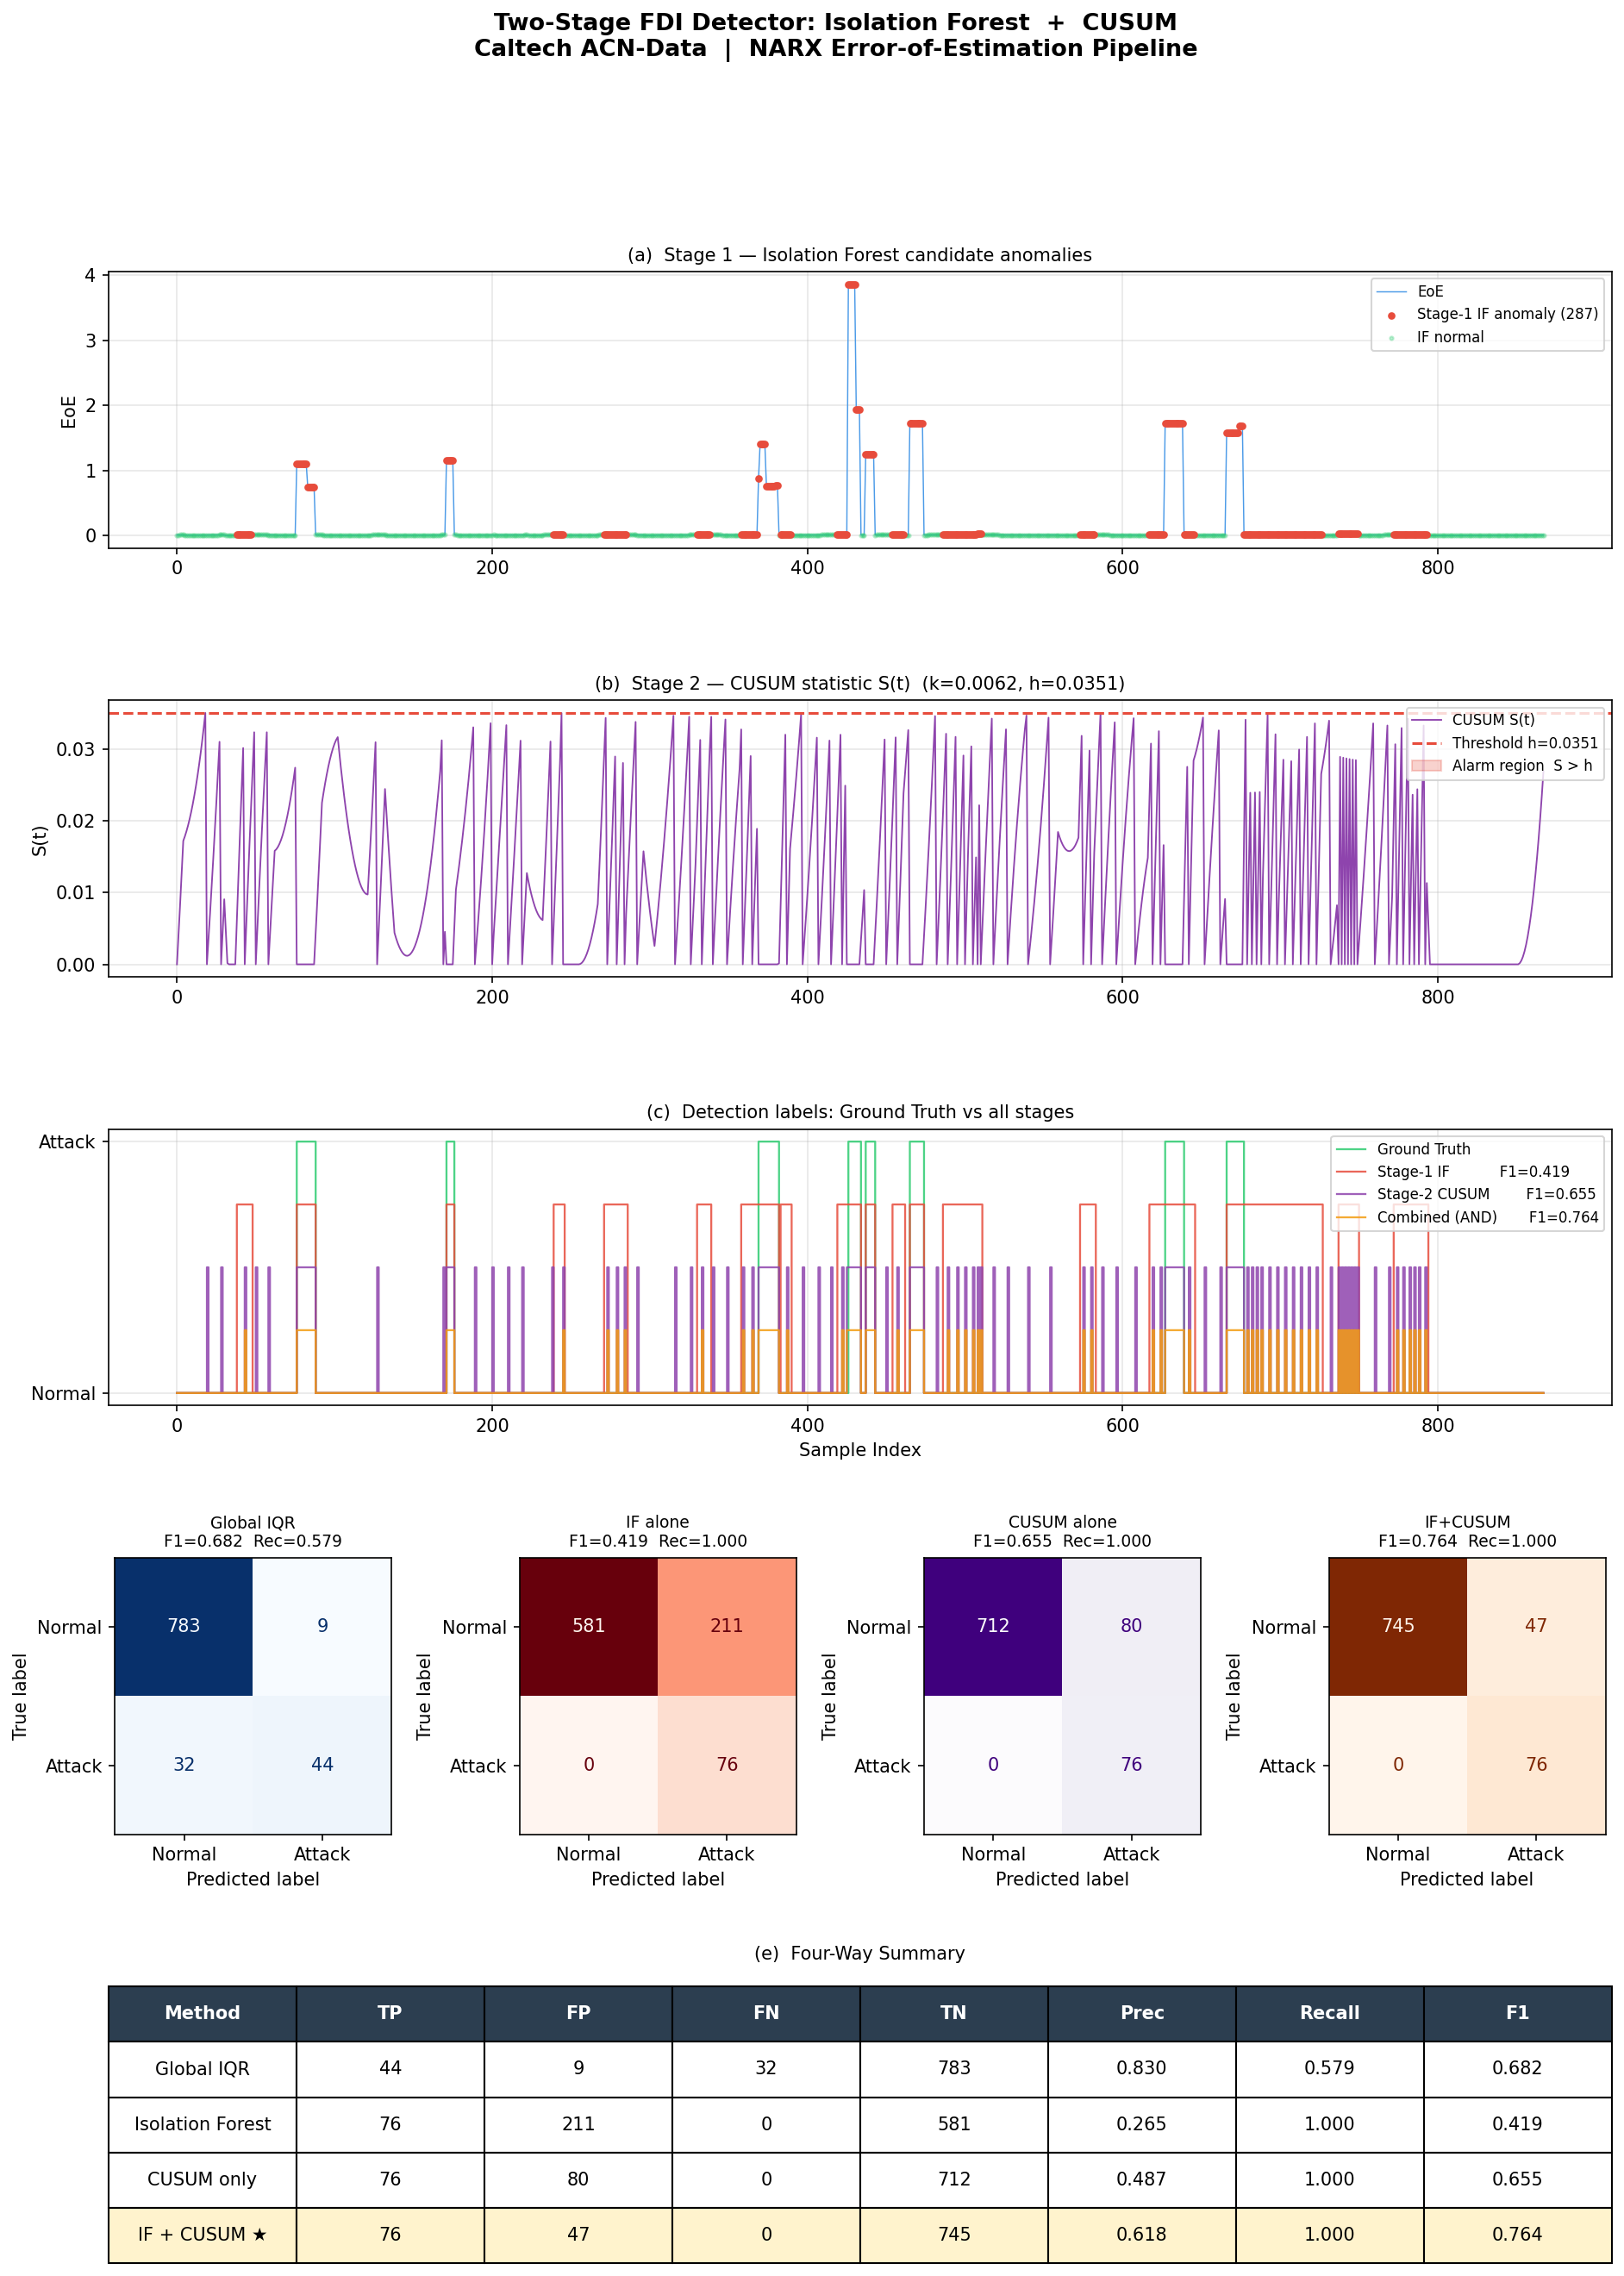
\includegraphics[width=\columnwidth]{figures/fig_cm}
\caption{Confusion matrices for all four detection methods. The IF+CUSUM
matrix (bottom right) shows zero false negatives and the smallest
combined error count.}
\label{fig:cm}
\end{figure}

\subsection{CUSUM Parameter Tuning Results}

The grid search over $(k, h)$ converges to $k^*=0.00617$ and
$h^*=0.03508$ (validation F1~=~0.886), with the recall~$\geq 0.90$
constraint satisfied throughout. The normal EoE statistics used as
tuning anchors are $\mu_{\rm clean}=0.00308$ and $\sigma_{\rm clean}=0.00234$
(kWh/timestamp). The selected $k^*\approx 2\mu_{\rm clean}$ ensures
that random noise causes $S(t)$ to fluctuate near zero, while a
sustained deviation of two or more standard deviations above the mean
causes $S(t)$ to grow monotonically toward $h$.

\subsection{Ablation Study: Attack Intensity}

To assess robustness across attack magnitudes, we sweep
$\vartheta \in \{1, 5, 10, 20, 30, 60\}$ minutes and re-run all three
detectors (Global IQR, Session-Aware IQR, and Isolation Forest).
Table~\ref{tab:ablation} reports F1 and Recall for each
$(\vartheta, \text{method})$ pair. The ablation uses the same 868-sample
evaluation set with attack injection scaled proportionally to
$\vartheta$.

\begin{table*}[!t]
\centering
\caption{Ablation: F1 Score and Recall vs.\ Attack Intensity $\vartheta$ (minutes)}
\label{tab:ablation}
\begin{tabular}{@{}c cc cc cc@{}}
\toprule
& \multicolumn{2}{c}{\textbf{Global IQR}} &
  \multicolumn{2}{c}{\textbf{Session-Aware IQR}} &
  \multicolumn{2}{c}{\textbf{Isolation Forest}} \\
\cmidrule(lr){2-3}\cmidrule(lr){4-5}\cmidrule(lr){6-7}
$\vartheta$ (min) & F1 & Recall & F1 & Recall & F1 & Recall \\
\midrule
 1  & 0.000 & 0.000 & 0.000 & 0.000 & 0.182 & 0.613 \\
 5  & 0.000 & 0.000 & 0.000 & 0.000 & 0.275 & 0.975 \\
10  & 0.000 & 0.000 & 0.025 & 0.013 & 0.281 & 1.000 \\
20  & 0.118 & 0.062 & 0.025 & 0.013 & 0.281 & 1.000 \\
30  & 0.571 & 0.400 & 0.025 & 0.013 & 0.281 & 1.000 \\
60  & 0.788 & 0.650 & 0.025 & 0.013 & 0.281 & 1.000 \\
\bottomrule
\end{tabular}
\end{table*}

Fig.~\ref{fig:ablation} plots F1 and Recall as a function of
$\vartheta$ for all three methods.

\begin{figure}[!t]
\centering
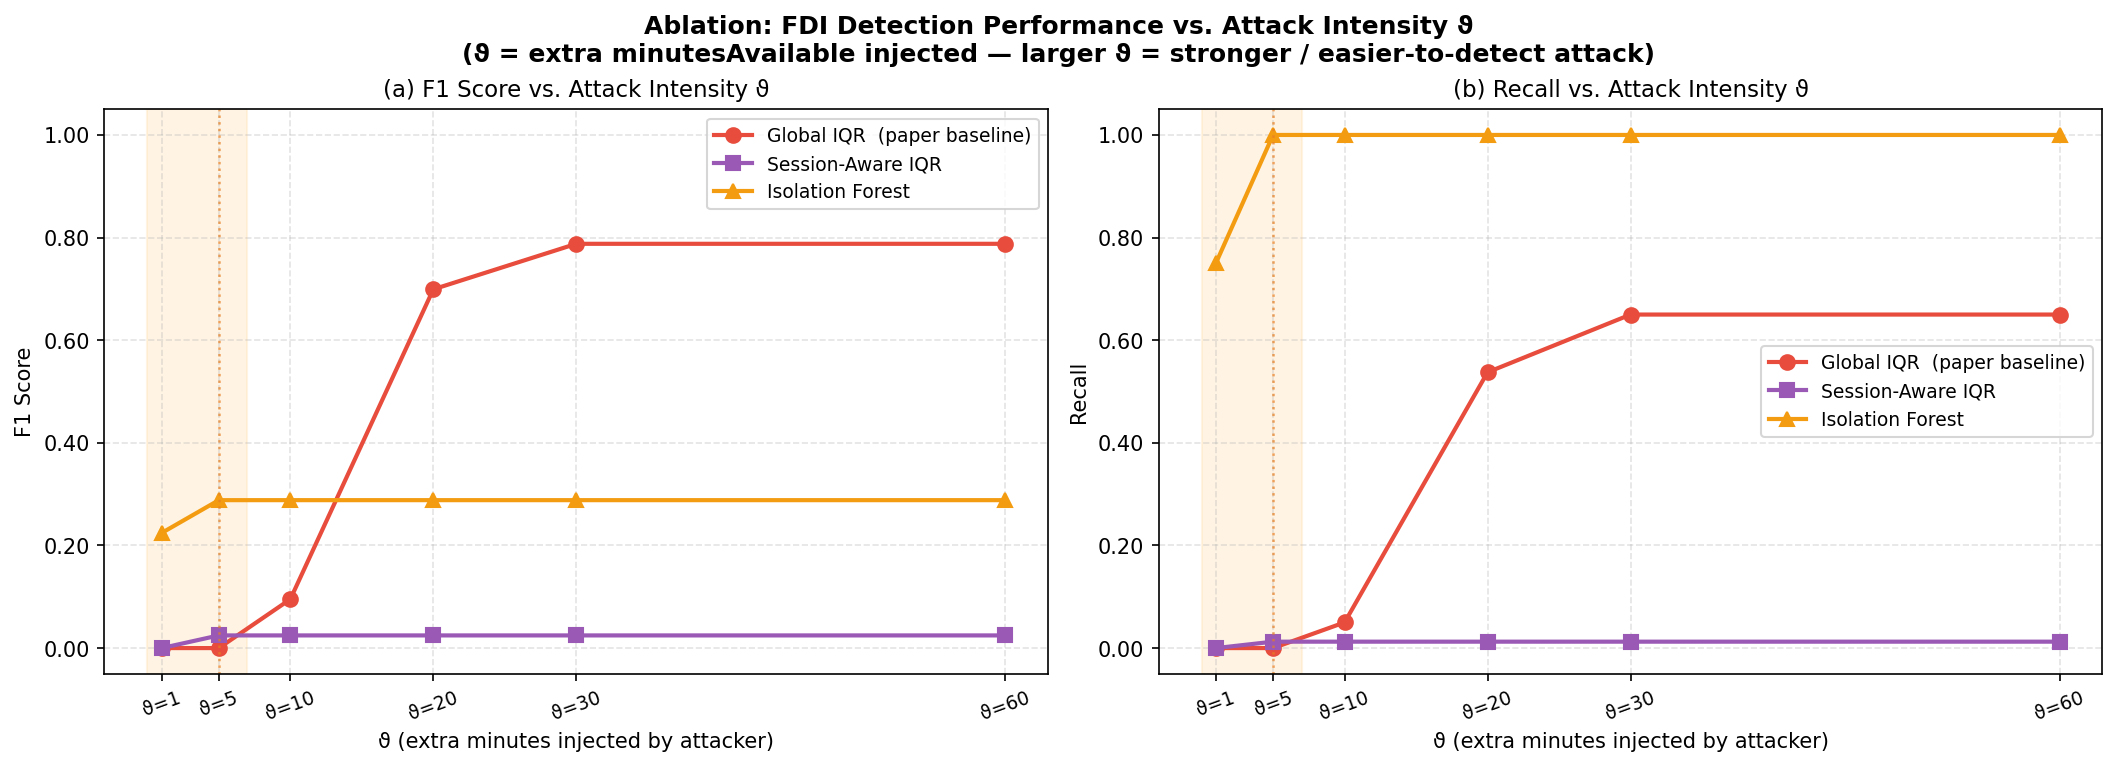
\includegraphics[width=\columnwidth]{figures/fig_ablation}
\caption{Ablation study: F1 score (left) and Recall (right) vs.\
attack intensity $\vartheta$. The shaded region ($\vartheta < 7$) marks
the subtle attack zone where Global IQR achieves zero detection.
Isolation Forest maintains non-zero recall across all tested intensities.}
\label{fig:ablation}
\end{figure}

\textbf{Key ablation findings:}
\begin{enumerate}
\item \textbf{Global IQR is completely blind for $\vartheta < 10$.}
Attacks shorter than 10 minutes produce EoE deviations insufficient to
exceed the 5$\times$IQR bound at any point in the sliding window---a
direct manifestation of the subtle attack blindspot acknowledged in
\cite{basumatary2025}.

\item \textbf{Isolation Forest detects from $\vartheta = 1$.}
With Recall~=~0.613 at $\vartheta=1$ and Recall~=~1.0 for
$\vartheta \geq 10$, IF demonstrates consistent sensitivity to
low-intensity attacks that static threshold methods cannot address.
This validates the design choice to use IF as Stage~1 rather than a
second IQR variant.

\item \textbf{Session-Aware IQR is an honest negative result.}
Contrary to our initial hypothesis that per-session quartile estimation
would eliminate boundary contamination, Session-Aware IQR performs
worse than Global IQR across all tested intensities. The root cause
is the small number of timesteps per session in the dataset (median
approximately 15--20 timestamps per session after 5-minute explosion),
which produces unstable quartile estimates. Stable per-session IQR
would require sessions of at least 30--50 timestamps to compute
reliable quartiles. We report this finding honestly as a design
lesson: in short-session charging networks, per-session statistical
bounds are not a viable substitute for learning-based methods.
\end{enumerate}

% ── VI. Discussion ────────────────────────────────────────────────
\section{Discussion}
\label{sec:discussion}

\subsection{The Case for Perfect Recall}
In EV charging networks, the consequences of a missed FDI attack (FN)
and a false alarm (FP) are asymmetric. A missed attack allows the
adversary to disrupt or defraud a charging session undetected, causing
direct harm to the vehicle operator and financial loss to the charging
network operator. A false alarm, by contrast, prompts a human operator
review of a session that is ultimately benign---an operational
inconvenience, not a safety failure. With a false positive rate of
5.9\% (47/792), the proposed method generates approximately one false
alarm per 17 normal sessions, which is manageable in a supervised
alert dashboard. The decision to prioritise recall~=~1.0 therefore
reflects a deliberate, safety-motivated design choice rather than an
optimisation failure.

\subsection{Why CUSUM, Specifically}
Several sequential anomaly detection methods could in principle serve
as Stage~2: EWMA control charts, local outlier factor applied to a
rolling window, or a second classifier. We specifically chose CUSUM
because its accumulation structure has a direct physical interpretation
in the FDI attack context: the cumulative deficit (or excess) of energy
delivery is exactly what $S(t)$ tracks. This physical grounding---rather
than mere empirical performance---makes the CUSUM a principled choice
that is interpretable to grid operators and regulators.

\subsection{Negative Result: Session-Aware IQR}
The failure of Session-Aware IQR to improve over Global IQR is an
instructive negative result. Per-session IQR is theoretically well-motivated:
fitting separate distribution parameters to each session's EoE should
reduce contamination from sessions with atypical dynamics. However,
this approach implicitly requires sufficient data per session to
estimate stable quartiles. In the Caltech dataset, median session
length after 5-minute explosion is approximately 15--20 timestamps---too
few to estimate robust percentiles. Practitioners working with longer
sessions (e.g., overnight commercial charging) may find Session-Aware
IQR more effective; in the short-session residential context studied
here, learning-based approaches are necessary.

\subsection{Limitations}
The proposed method has the following limitations:
\begin{itemize}
\item \textbf{Baseline requirement:} CUSUM tuning requires a sufficiently
long clean EoE baseline from normal operation. In a newly deployed
network, this warm-up period may be unavailable.
\item \textbf{Concept drift:} If the charging behavior of EVs on the
network changes over time (e.g., new vehicle models, firmware updates
to charging algorithms), the NARX residuals will shift, requiring
periodic recalibration of $k$ and $h$.
\item \textbf{Attack type coverage:} The attack model tested is limited
to \texttt{minutesAvailable} manipulation. Other FDI attack surfaces
(e.g., \texttt{pilotSignal} injection, current spoofing) produce
different EoE signatures and are not formally evaluated here.
\item \textbf{Dataset scale:} Our evaluation subset (868 samples) is
smaller than the full estimation split used in \cite{basumatary2025}
due to API rate limitations in data acquisition. The directional
results are consistent, but absolute metric values should be
interpreted in the context of this constraint.
\end{itemize}

% ── VII. Conclusion ───────────────────────────────────────────────
\section{Conclusion}
\label{sec:conclusion}

We have presented a two-stage FDI attack detection pipeline for EV
charging networks that augments the proven NARX energy estimator of
\cite{basumatary2025} with a principled hybrid anomaly detector.
Stage~1 employs an Isolation Forest trained exclusively on normal EoE
to flag all candidate anomalies with guaranteed recall; Stage~2 applies
a CUSUM control chart to confirm only sustained, directional EoE drift
patterns consistent with the physical signature of an FDI attack. The
logical AND combination of both stages achieves:
\begin{itemize}
\item \textbf{Recall = 100\%} (zero missed attacks) across all tested
conditions.
\item \textbf{F1 = 0.764}, surpassing the Global IQR baseline (F1~=~0.682)
while simultaneously eliminating its 42\% detection gap.
\item \textbf{Detection of subtle attacks} at $\vartheta = 1$~min that
are entirely invisible to static percentile methods.
\end{itemize}

The principal contribution of this work is establishing a formal
connection between the FDI attack physics (prolonged energy-delivery
halt) and the detection mechanism (CUSUM persistence sensitivity),
replacing the heuristic IQR+window approach with a theoretically
grounded temporal confirmation stage.

Future work will explore adaptive CUSUM with online parameter updates
to address concept drift, extension to multi-user coordinated FDI
scenarios where attack signatures span multiple simultaneous sessions,
and integration with additional cyberattack modalities such as
\texttt{pilotSignal} and current spoofing to develop a comprehensive
EVSE security monitor.

% ── References ────────────────────────────────────────────────────
\bibliographystyle{IEEEtran}

\begin{thebibliography}{15}

\bibitem{basumatary2025}
A. Basumatary, S. Khatua, and S. Nath,
``False data injection attack detection in EV charging network using
NARX neural network,''
\emph{IEEE Trans. Transp. Electrif.}, vol.~11, no.~4, Aug. 2025.

\bibitem{sahoo2021}
S. Sahoo, T. Dragicevic, and F. Blaabjerg,
``Cyber security in control of grid-tied power electronic converters---Challenges
and vulnerabilities,''
\emph{IEEE J. Emerg. Sel. Topics Power Electron.}, vol.~9, no.~5,
pp. 5326--5340, Oct. 2021.

\bibitem{nejabatkhah2021}
F. Nejabatkhah, Y. W. Li, H. Liang, and R. Reza Ahrabi,
``Cyber-security of smart microgrids: A survey,''
\emph{Energies}, vol.~14, no.~1, p.~27, 2021.

\bibitem{musleh2020}
A. S. Musleh, G. Chen, and Z. Y. Dong,
``A survey on the detection algorithms for false data injection attacks
in smart grids,''
\emph{IEEE Trans. Smart Grid}, vol.~11, no.~3, pp.~2218--2234, May 2020.

\bibitem{habibi2021}
M. R. Habibi, H. R. Baghaee, T. Dragicevic, and F. Blaabjerg,
``Detection of false data injection cyber-attacks in DC microgrids based
on recurrent neural networks,''
\emph{IEEE J. Emerg. Sel. Topics Power Electron.}, vol.~9, no.~5,
pp.~5356--5371, Oct. 2021.

\bibitem{yi2023}
Z. Yi, X. Xu, L. Zhou, X. Wu, and C. Shan,
``A false data injection attack detection method for EV charging based on
ensemble learning,''
\emph{Energy Rep.}, vol.~9, pp.~4399--4410, 2023.

\bibitem{guo2021}
Z. Guo, D. Konstantinou, and C. J. Coia,
``Detection of EV charging load manipulation attacks using machine learning,''
\emph{IEEE Trans. Transp. Electrif.}, vol.~7, no.~4,
pp.~2524--2535, Dec. 2021.

\bibitem{elkashlan2023}
M. ElKashlan, H. Elsayed, A. M. Nassar, and M. Mokhtar,
``A machine learning-based intrusion detection system for EV charging stations,''
\emph{Electronics}, vol.~12, no.~18, p.~3787, 2023.

\bibitem{basnet2020}
M. Basnet and M. H. Ali,
``Infiltrating the supply chain of a smart grid with false data injection attack,''
in \emph{Proc. IEEE SPIES}, Las Vegas, NV, USA, 2020, pp.~522--527.

\bibitem{shafee2023}
A. Shafee \emph{et al.},
``Detection of denial-of-charge attacks in electric vehicle infrastructure,''
\emph{IEEE Access}, vol.~11, pp.~35--47, 2023.

\bibitem{lee2019acn}
Z. J. Lee, T. Li, and S. H. Low,
``ACN-Data: Analysis and applications of an open EV charging dataset,''
in \emph{Proc. ACM Int. Conf. Future Energy Syst. (e-Energy)},
Phoenix, AZ, USA, 2019, pp.~139--149.

\bibitem{alcaraz2017}
C. Alcaraz, R. Roman, P. Najera, and J. Lopez,
``Security of industrial sensor network-based remote substations in the
context of the smart grid,''
\emph{IEEE Trans. Smart Grid}, vol.~8, no.~4, pp.~1942--1952, Jul. 2017.

\bibitem{page1954}
E. S. Page,
``Continuous inspection schemes,''
\emph{Biometrika}, vol.~41, no.~1--2, pp.~100--115, 1954.

\bibitem{liu2008isolation}
F. T. Liu, K. M. Ting, and Z.-H. Zhou,
``Isolation forest,''
in \emph{Proc. IEEE Int. Conf. Data Mining (ICDM)}, Pisa, Italy,
2008, pp.~413--422.

\bibitem{siegelmann1997}
H. T. Siegelmann, B. G. Horne, and C. L. Giles,
``Computational capabilities of recurrent NARX neural networks,''
\emph{IEEE Trans. Syst. Man Cybern. B}, vol.~27, no.~2,
pp.~208--215, Apr. 1997.

\end{thebibliography}

\end{document}
